\documentclass{book}
\usepackage[a4paper,top=2.5cm,bottom=2.5cm,left=2.5cm,right=2.5cm]{geometry}
\usepackage{makeidx}
\usepackage{natbib}
\usepackage{graphicx}
\usepackage{multicol}
\usepackage{float}
\usepackage{listings}
\usepackage{color}
\usepackage{ifthen}
\usepackage[table]{xcolor}
\usepackage{textcomp}
\usepackage{alltt}
\usepackage{ifpdf}
\ifpdf
\usepackage[pdftex,
            pagebackref=true,
            colorlinks=true,
            linkcolor=blue,
            unicode
           ]{hyperref}
\else
\usepackage[ps2pdf,
            pagebackref=true,
            colorlinks=true,
            linkcolor=blue,
            unicode
           ]{hyperref}
\usepackage{pspicture}
\fi
\usepackage[utf8]{inputenc}
\usepackage{polski}
\usepackage[T1]{fontenc}

\usepackage{mathptmx}
\usepackage[scaled=.90]{helvet}
\usepackage{courier}
\usepackage{sectsty}
\usepackage{amssymb}
\usepackage[titles]{tocloft}
\usepackage{doxygen}
\lstset{language=C++,inputencoding=utf8,basicstyle=\footnotesize,breaklines=true,breakatwhitespace=true,tabsize=4,numbers=left }
\makeindex
\setcounter{tocdepth}{3}
\renewcommand{\footrulewidth}{0.4pt}
\renewcommand{\familydefault}{\sfdefault}
\hfuzz=15pt
\setlength{\emergencystretch}{15pt}
\hbadness=750
\tolerance=750
\begin{document}
\hypersetup{pageanchor=false,citecolor=blue}
\begin{titlepage}
\vspace*{7cm}
\begin{center}
{\Large Dokumentacja laboratorium P\-S\-S }\\
\vspace*{1cm}
{\large Wygenerowano przez Doxygen 1.8.2}\\
\vspace*{0.5cm}
{\small Wt, 25 kwi 2023 21:05:21}\\
\end{center}
\end{titlepage}
\clearemptydoublepage
\pagenumbering{roman}
\tableofcontents
\clearemptydoublepage
\pagenumbering{arabic}
\hypersetup{pageanchor=true,citecolor=blue}
\chapter{Dokumentacja Laboratorium P\-S\-S}
\label{md_README}
\hypertarget{md_README}{}
Dokumentacja projektu wykonywanego w ramach kursu PSS, polegającego na symulacji obiektu dyskrytnego.\hypertarget{md__r_e_a_d_m_e_autotoc_md1}{}\doxysection{Autor}\label{md__r_e_a_d_m_e_autotoc_md1}
Szymon Lubszczyk \hypertarget{md__r_e_a_d_m_e_autotoc_md2}{}\doxysection{Zawartość}\label{md__r_e_a_d_m_e_autotoc_md2}
Kod źrodłowy poszczególnych elementów, wchodzących w skład projektu z opisem i komentarzami. 
\chapter{Indeks hierarchiczny}
\doxysection{Hierarchia klas}
Ta lista dziedziczenia posortowana jest z grubsza, choć nie całkowicie, alfabetycznie\+:\begin{DoxyCompactList}
\item \contentsline{section}{SISO}{\pageref{class_s_i_s_o}}{}
\begin{DoxyCompactList}
\item \contentsline{section}{ARX}{\pageref{class_a_r_x}}{}
\item \contentsline{section}{PD}{\pageref{class_p_d}}{}
\begin{DoxyCompactList}
\item \contentsline{section}{PID}{\pageref{class_p_i_d}}{}
\end{DoxyCompactList}
\item \contentsline{section}{PI}{\pageref{class_p_i}}{}
\begin{DoxyCompactList}
\item \contentsline{section}{PID}{\pageref{class_p_i_d}}{}
\end{DoxyCompactList}
\end{DoxyCompactList}
\end{DoxyCompactList}

\chapter{Indeks klas}
\section{Lista klas}
Tutaj znajdują się klasy, struktury, unie i interfejsy wraz z ich krótkimi opisami\-:\begin{DoxyCompactList}
\item\contentsline{section}{\hyperlink{class_a_r_x}{A\-R\-X} }{\pageref{class_a_r_x}}{}
\item\contentsline{section}{\hyperlink{class_s_i_s_o}{S\-I\-S\-O} }{\pageref{class_s_i_s_o}}{}
\end{DoxyCompactList}

\chapter{Indeks plików}
\doxysection{Lista plików}
Tutaj znajduje się lista wszystkich plików z ich krótkimi opisami\+:\begin{DoxyCompactList}
\item\contentsline{section}{\mbox{\hyperlink{_dekorator_8cpp}{Dekorator.\+cpp}} }{\pageref{_dekorator_8cpp}}{}
\item\contentsline{section}{\mbox{\hyperlink{_dekorator_8hpp}{Dekorator.\+hpp}} }{\pageref{_dekorator_8hpp}}{}
\item\contentsline{section}{\mbox{\hyperlink{_dek_prost_8cpp}{Dek\+Prost.\+cpp}} }{\pageref{_dek_prost_8cpp}}{}
\item\contentsline{section}{\mbox{\hyperlink{_dek_prost_8hpp}{Dek\+Prost.\+hpp}} }{\pageref{_dek_prost_8hpp}}{}
\item\contentsline{section}{\mbox{\hyperlink{_dek_sin_8cpp}{Dek\+Sin.\+cpp}} }{\pageref{_dek_sin_8cpp}}{}
\item\contentsline{section}{\mbox{\hyperlink{_dek_sin_8hpp}{Dek\+Sin.\+hpp}} }{\pageref{_dek_sin_8hpp}}{}
\item\contentsline{section}{\mbox{\hyperlink{_dek_szum_8cpp}{Dek\+Szum.\+cpp}} }{\pageref{_dek_szum_8cpp}}{}
\item\contentsline{section}{\mbox{\hyperlink{_dek_szum_8hpp}{Dek\+Szum.\+hpp}} }{\pageref{_dek_szum_8hpp}}{}
\item\contentsline{section}{\mbox{\hyperlink{funkcje_pomocnicze_8cpp}{funkcje\+Pomocnicze.\+cpp}} }{\pageref{funkcje_pomocnicze_8cpp}}{}
\item\contentsline{section}{\mbox{\hyperlink{funkcje_pomocniczne_8hpp}{funkcje\+Pomocniczne.\+hpp}} }{\pageref{funkcje_pomocniczne_8hpp}}{}
\item\contentsline{section}{\mbox{\hyperlink{klasa_a_r_x_8cpp}{klasa\+ARX.\+cpp}} }{\pageref{klasa_a_r_x_8cpp}}{}
\item\contentsline{section}{\mbox{\hyperlink{klasa_a_r_x_8hpp}{klasa\+ARX.\+hpp}} }{\pageref{klasa_a_r_x_8hpp}}{}
\item\contentsline{section}{\mbox{\hyperlink{klasa_s_i_s_o_8hpp}{klasa\+SISO.\+hpp}} }{\pageref{klasa_s_i_s_o_8hpp}}{}
\item\contentsline{section}{\mbox{\hyperlink{_komponent_8hpp}{Komponent.\+hpp}} }{\pageref{_komponent_8hpp}}{}
\item\contentsline{section}{\mbox{\hyperlink{_komponent___struktura_8hpp}{Komponent\+\_\+\+Struktura.\+hpp}} }{\pageref{_komponent___struktura_8hpp}}{}
\item\contentsline{section}{\mbox{\hyperlink{_komponent_konkretny_8hpp}{Komponent\+Konkretny.\+hpp}} }{\pageref{_komponent_konkretny_8hpp}}{}
\item\contentsline{section}{\mbox{\hyperlink{_kompozyt_8hpp}{Kompozyt.\+hpp}} }{\pageref{_kompozyt_8hpp}}{}
\item\contentsline{section}{\mbox{\hyperlink{_komp_row_8cpp}{Komp\+Row.\+cpp}} }{\pageref{_komp_row_8cpp}}{}
\item\contentsline{section}{\mbox{\hyperlink{_komp_row_8hpp}{Komp\+Row.\+hpp}} }{\pageref{_komp_row_8hpp}}{}
\item\contentsline{section}{\mbox{\hyperlink{_komp_sz_8cpp}{Komp\+Sz.\+cpp}} }{\pageref{_komp_sz_8cpp}}{}
\item\contentsline{section}{\mbox{\hyperlink{_komp_sz_8hpp}{Komp\+Sz.\+hpp}} }{\pageref{_komp_sz_8hpp}}{}
\item\contentsline{section}{\mbox{\hyperlink{_obiekt_dyskretny_lab_8cpp}{Obiekt\+Dyskretny\+Lab.\+cpp}} }{\pageref{_obiekt_dyskretny_lab_8cpp}}{}
\item\contentsline{section}{\mbox{\hyperlink{_p_d_8cpp}{PD.\+cpp}} }{\pageref{_p_d_8cpp}}{}
\item\contentsline{section}{\mbox{\hyperlink{_p_d_8hpp}{PD.\+hpp}} }{\pageref{_p_d_8hpp}}{}
\item\contentsline{section}{\mbox{\hyperlink{_p_i_8cpp}{PI.\+cpp}} }{\pageref{_p_i_8cpp}}{}
\item\contentsline{section}{\mbox{\hyperlink{_p_i_8hpp}{PI.\+hpp}} }{\pageref{_p_i_8hpp}}{}
\item\contentsline{section}{\mbox{\hyperlink{_p_i_d_8cpp}{PID.\+cpp}} }{\pageref{_p_i_d_8cpp}}{}
\item\contentsline{section}{\mbox{\hyperlink{_p_i_d_8hpp}{PID.\+hpp}} }{\pageref{_p_i_d_8hpp}}{}
\end{DoxyCompactList}

\chapter{Dokumentacja klas}
\hypertarget{class_a_r_x}{}\doxysection{Dokumentacja klasy ARX}
\label{class_a_r_x}\index{ARX@{ARX}}


{\ttfamily \#include $<$klasa\+ARX.\+hpp$>$}

Diagram dziedziczenia dla ARX\begin{figure}[H]
\begin{center}
\leavevmode
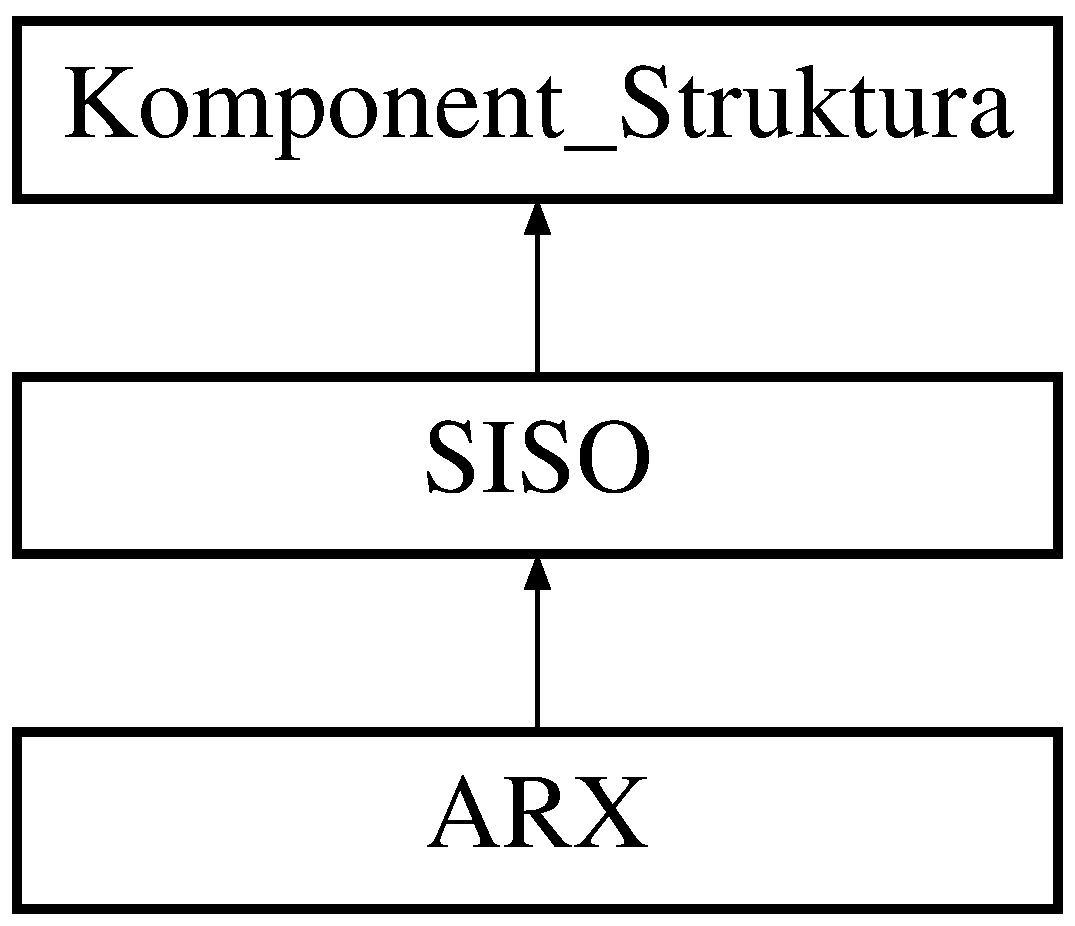
\includegraphics[height=3.000000cm]{class_a_r_x}
\end{center}
\end{figure}
\doxysubsection*{Metody publiczne}
\begin{DoxyCompactItemize}
\item 
\mbox{\hyperlink{class_a_r_x_a33446ecffef6c604cae4b0376dc90d30}{ARX}} ()
\begin{DoxyCompactList}\small\item\em Konstruktor domyślny. \end{DoxyCompactList}\item 
\mbox{\hyperlink{class_a_r_x_a66d58bf40e241b9c764f63aacdb96feb}{ARX}} (std\+::vector$<$ double $>$ nparamA, std\+::vector$<$ double $>$ nparamB, unsigned int nk, double nvarE)
\item 
\mbox{\hyperlink{class_a_r_x_abbba12ab36a3f0a6536938b242271c9f}{$\sim$\+ARX}} ()
\item 
std\+::ostream \& \mbox{\hyperlink{class_a_r_x_a8660da07ee58cf49db7bcf61affbf568}{wyswietl\+Parametry}} (std\+::ostream \&os)
\begin{DoxyCompactList}\small\item\em Metoda odpowiedzialna za wyświetlenie aktualnych pól opisujących model \mbox{\hyperlink{class_a_r_x}{ARX}}. \end{DoxyCompactList}\item 
void \mbox{\hyperlink{class_a_r_x_a0ea5d18350bae9be968171e5f2077d0f}{aktualizuj\+WielomianA}} (std\+::vector$<$ double $>$ wielomian)
\begin{DoxyCompactList}\small\item\em Zmiana współczynników wielomianu A. \end{DoxyCompactList}\item 
void \mbox{\hyperlink{class_a_r_x_abaef0e431556e7a22180c35b2306a55a}{aktualizuj\+WielomianB}} (std\+::vector$<$ double $>$ wielomian)
\begin{DoxyCompactList}\small\item\em Zmiana współczynników wielomianu B. \end{DoxyCompactList}\item 
void \mbox{\hyperlink{class_a_r_x_a940f5087455d8d6ce64e27b36a0fdc7e}{aktualizuj\+Parametr}} (unsigned int parametr)
\begin{DoxyCompactList}\small\item\em Zmiana opóźnienia modelu \mbox{\hyperlink{class_a_r_x}{ARX}}. \end{DoxyCompactList}\item 
void \mbox{\hyperlink{class_a_r_x_a6353c1891e1b8ad9fa62ec14536caaa1}{aktualizuj\+Parametr}} (double parametr)
\begin{DoxyCompactList}\small\item\em Zmiana wariancji białego szumu. \end{DoxyCompactList}\item 
double \mbox{\hyperlink{class_a_r_x_aa2ee25b5f56aa74bda0323f61cef3c27}{Symuluj}} (double \mbox{\hyperlink{class_a_r_x_af61ad06d76ce7b19daa55ee0f59639e7}{s\+\_\+u}}) override
\begin{DoxyCompactList}\small\item\em Dziedziczona metoda Symuluj z klasy bazowej \mbox{\hyperlink{class_s_i_s_o}{SISO}}. \end{DoxyCompactList}\item 
void \mbox{\hyperlink{class_a_r_x_a31e36511ddebb81a49d6bb82e086dda7}{odczytaj\+Dane}} (\mbox{\hyperlink{class_a_r_x}{ARX}} \&arx, const std\+::string \&file\+\_\+path)
\item 
void \mbox{\hyperlink{class_a_r_x_a1b6183dbda8b9224847f691bd2eff93d}{zapisz\+Dane}} (const std\+::string \&file\+\_\+path)
\end{DoxyCompactItemize}
\doxysubsubsection*{Metody publiczne dziedziczone z \mbox{\hyperlink{class_s_i_s_o}{SISO}}}
\begin{DoxyCompactItemize}
\item 
virtual \mbox{\hyperlink{class_s_i_s_o_a3f6b0b7cda79493b941553e5d5780167}{$\sim$\+SISO}} ()
\begin{DoxyCompactList}\small\item\em Przez to, że klasa posiada jedynie metodę wirtualną, wirtualny musi być również destruktor. \end{DoxyCompactList}\end{DoxyCompactItemize}
\doxysubsubsection*{Metody publiczne dziedziczone z \mbox{\hyperlink{class_komponent___struktura}{Komponent\+\_\+\+Struktura}}}
\begin{DoxyCompactItemize}
\item 
virtual \mbox{\hyperlink{class_komponent___struktura_a3df8c1a1177bda3f17857ecef6ba2d6d}{$\sim$\+Komponent\+\_\+\+Struktura}} ()
\begin{DoxyCompactList}\small\item\em Wirtualny destruktor. \end{DoxyCompactList}\item 
void \mbox{\hyperlink{class_komponent___struktura_a0b11947c38aed479c984c20d32cc77c0}{Set\+Parent}} (\mbox{\hyperlink{class_komponent___struktura}{Komponent\+\_\+\+Struktura}} $\ast$nparent)
\begin{DoxyCompactList}\small\item\em Ustawienie danego \char`\"{}rodzica\char`\"{}. \end{DoxyCompactList}\item 
\mbox{\hyperlink{class_komponent___struktura}{Komponent\+\_\+\+Struktura}} $\ast$ \mbox{\hyperlink{class_komponent___struktura_a5eb3e69b28b2fb3ad8d761611a3e8927}{Get\+Parent}} () const
\begin{DoxyCompactList}\small\item\em Odebranie danego rodzica. \end{DoxyCompactList}\item 
virtual void \mbox{\hyperlink{class_komponent___struktura_afbe374b319f9be537bd65250173c0190}{dodaj}} (\mbox{\hyperlink{class_komponent___struktura}{Komponent\+\_\+\+Struktura}} $\ast$komponent)
\begin{DoxyCompactList}\small\item\em Operacja dodawania kolejnych \char`\"{}dzieci\char`\"{} do drzewa. W tym wypadku s� to obiekty \mbox{\hyperlink{class_s_i_s_o}{SISO}}. \end{DoxyCompactList}\item 
virtual void \mbox{\hyperlink{class_komponent___struktura_a9ebab0e681403b17baa7b9ba2579ecaa}{usun}} (\mbox{\hyperlink{class_komponent___struktura}{Komponent\+\_\+\+Struktura}} $\ast$komponent)
\begin{DoxyCompactList}\small\item\em Operacja usuni�cia kolejnych \char`\"{}dzieci\char`\"{} do drzewa. W tym wypadku s� to obiekty \mbox{\hyperlink{class_s_i_s_o}{SISO}}. \end{DoxyCompactList}\item 
virtual double \mbox{\hyperlink{class_komponent___struktura_a19686e69b56cee733d792af23e9237b7}{Symuluj}} (double s\+\_\+u)=0
\end{DoxyCompactItemize}
\doxysubsection*{Atrybuty chronione}
\begin{DoxyCompactItemize}
\item 
std\+::vector$<$ double $>$ \mbox{\hyperlink{class_a_r_x_a6f9a9743a50d912f9e8547a433b2baea}{s\+\_\+paramA}}
\begin{DoxyCompactList}\small\item\em Współczynniki wielomianu A. \end{DoxyCompactList}\item 
std\+::vector$<$ double $>$ \mbox{\hyperlink{class_a_r_x_a57104d29d3cdd002f814d3460a9be2df}{s\+\_\+paramB}}
\begin{DoxyCompactList}\small\item\em Współczynniki wielomianu B. \end{DoxyCompactList}\item 
std\+::deque$<$ double $>$ \mbox{\hyperlink{class_a_r_x_af61ad06d76ce7b19daa55ee0f59639e7}{s\+\_\+u}}
\begin{DoxyCompactList}\small\item\em Kolejka z wartościami wejścia. Jej rozmiar zależy od ilości współczynników wielomianu B zsumowaną z opóźnieniem. \end{DoxyCompactList}\item 
std\+::deque$<$ double $>$ \mbox{\hyperlink{class_a_r_x_aaeb3515374c95f4b7ed58c9676d89639}{s\+\_\+y}}
\begin{DoxyCompactList}\small\item\em Kolejka z wartościami wyjścia. Jej rozmiar zależy od ilości współczynników wielomianu A. \end{DoxyCompactList}\end{DoxyCompactItemize}
\doxysubsubsection*{Atrybuty chronione dziedziczone z \mbox{\hyperlink{class_komponent___struktura}{Komponent\+\_\+\+Struktura}}}
\begin{DoxyCompactItemize}
\item 
\mbox{\hyperlink{class_komponent___struktura}{Komponent\+\_\+\+Struktura}} $\ast$ \mbox{\hyperlink{class_komponent___struktura_a7cb0e2ed12c6c2ecdfde465b1f1f4b54}{parent}}
\begin{DoxyCompactList}\small\item\em Wska�nik na klas� \mbox{\hyperlink{class_komponent___struktura}{Komponent\+\_\+\+Struktura}} wskazuj�ca na \char`\"{}rodzic�w\char`\"{}, czyli najstarsze elementy drzewa. \end{DoxyCompactList}\end{DoxyCompactItemize}
\doxysubsection*{Atrybuty prywatne}
\begin{DoxyCompactItemize}
\item 
unsigned int \mbox{\hyperlink{class_a_r_x_a7d9974f04433a984d5562c7c403e102a}{s\+\_\+k}}
\begin{DoxyCompactList}\small\item\em Opóźnienie. \end{DoxyCompactList}\item 
double \mbox{\hyperlink{class_a_r_x_a3361b14c8d2d075a3c23e7d2f07c8592}{s\+\_\+varE}}
\begin{DoxyCompactList}\small\item\em Wariancja białego szumu. \end{DoxyCompactList}\end{DoxyCompactItemize}


\doxysubsection{Opis szczegółowy}


Definicja w linii \mbox{\hyperlink{klasa_a_r_x_8hpp_source_l00012}{12}} pliku \mbox{\hyperlink{klasa_a_r_x_8hpp_source}{klasa\+ARX.\+hpp}}.



\doxysubsection{Dokumentacja konstruktora i destruktora}
\mbox{\Hypertarget{class_a_r_x_a33446ecffef6c604cae4b0376dc90d30}\label{class_a_r_x_a33446ecffef6c604cae4b0376dc90d30}} 
\index{ARX@{ARX}!ARX@{ARX}}
\index{ARX@{ARX}!ARX@{ARX}}
\doxysubsubsection{\texorpdfstring{ARX()}{ARX()}\hspace{0.1cm}{\footnotesize\ttfamily [1/2]}}
{\footnotesize\ttfamily ARX\+::\+ARX (\begin{DoxyParamCaption}{ }\end{DoxyParamCaption})}



Konstruktor domyślny. 



Definicja w linii \mbox{\hyperlink{klasa_a_r_x_8cpp_source_l00020}{20}} pliku \mbox{\hyperlink{klasa_a_r_x_8cpp_source}{klasa\+ARX.\+cpp}}.

\mbox{\Hypertarget{class_a_r_x_a66d58bf40e241b9c764f63aacdb96feb}\label{class_a_r_x_a66d58bf40e241b9c764f63aacdb96feb}} 
\index{ARX@{ARX}!ARX@{ARX}}
\index{ARX@{ARX}!ARX@{ARX}}
\doxysubsubsection{\texorpdfstring{ARX()}{ARX()}\hspace{0.1cm}{\footnotesize\ttfamily [2/2]}}
{\footnotesize\ttfamily ARX\+::\+ARX (\begin{DoxyParamCaption}\item[{std\+::vector$<$ double $>$}]{nparamA,  }\item[{std\+::vector$<$ double $>$}]{nparamB,  }\item[{unsigned int}]{nk,  }\item[{double}]{nvarE }\end{DoxyParamCaption})}

Konstruktor parametryczny z następującymi zmiennymi wejściowymi\+: 
\begin{DoxyParams}[1]{Parametry}
\mbox{\texttt{ in}}  & {\em paramA} & \\
\hline
\mbox{\texttt{ in}}  & {\em paramB} & \\
\hline
\mbox{\texttt{ in}}  & {\em k} & \\
\hline
\mbox{\texttt{ in}}  & {\em varE} & \\
\hline
\end{DoxyParams}


Definicja w linii \mbox{\hyperlink{klasa_a_r_x_8cpp_source_l00027}{27}} pliku \mbox{\hyperlink{klasa_a_r_x_8cpp_source}{klasa\+ARX.\+cpp}}.

\mbox{\Hypertarget{class_a_r_x_abbba12ab36a3f0a6536938b242271c9f}\label{class_a_r_x_abbba12ab36a3f0a6536938b242271c9f}} 
\index{ARX@{ARX}!````~ARX@{$\sim$ARX}}
\index{````~ARX@{$\sim$ARX}!ARX@{ARX}}
\doxysubsubsection{\texorpdfstring{$\sim$ARX()}{~ARX()}}
{\footnotesize\ttfamily ARX\+::$\sim$\+ARX (\begin{DoxyParamCaption}{ }\end{DoxyParamCaption})}



Definicja w linii \mbox{\hyperlink{klasa_a_r_x_8cpp_source_l00032}{32}} pliku \mbox{\hyperlink{klasa_a_r_x_8cpp_source}{klasa\+ARX.\+cpp}}.



\doxysubsection{Dokumentacja funkcji składowych}
\mbox{\Hypertarget{class_a_r_x_a6353c1891e1b8ad9fa62ec14536caaa1}\label{class_a_r_x_a6353c1891e1b8ad9fa62ec14536caaa1}} 
\index{ARX@{ARX}!aktualizujParametr@{aktualizujParametr}}
\index{aktualizujParametr@{aktualizujParametr}!ARX@{ARX}}
\doxysubsubsection{\texorpdfstring{aktualizujParametr()}{aktualizujParametr()}\hspace{0.1cm}{\footnotesize\ttfamily [1/2]}}
{\footnotesize\ttfamily void ARX\+::aktualizuj\+Parametr (\begin{DoxyParamCaption}\item[{double}]{parametr }\end{DoxyParamCaption})}



Zmiana wariancji białego szumu. 



Definicja w linii \mbox{\hyperlink{klasa_a_r_x_8cpp_source_l00091}{91}} pliku \mbox{\hyperlink{klasa_a_r_x_8cpp_source}{klasa\+ARX.\+cpp}}.

\mbox{\Hypertarget{class_a_r_x_a940f5087455d8d6ce64e27b36a0fdc7e}\label{class_a_r_x_a940f5087455d8d6ce64e27b36a0fdc7e}} 
\index{ARX@{ARX}!aktualizujParametr@{aktualizujParametr}}
\index{aktualizujParametr@{aktualizujParametr}!ARX@{ARX}}
\doxysubsubsection{\texorpdfstring{aktualizujParametr()}{aktualizujParametr()}\hspace{0.1cm}{\footnotesize\ttfamily [2/2]}}
{\footnotesize\ttfamily void ARX\+::aktualizuj\+Parametr (\begin{DoxyParamCaption}\item[{unsigned int}]{parametr }\end{DoxyParamCaption})}



Zmiana opóźnienia modelu \mbox{\hyperlink{class_a_r_x}{ARX}}. 



Definicja w linii \mbox{\hyperlink{klasa_a_r_x_8cpp_source_l00080}{80}} pliku \mbox{\hyperlink{klasa_a_r_x_8cpp_source}{klasa\+ARX.\+cpp}}.

\mbox{\Hypertarget{class_a_r_x_a0ea5d18350bae9be968171e5f2077d0f}\label{class_a_r_x_a0ea5d18350bae9be968171e5f2077d0f}} 
\index{ARX@{ARX}!aktualizujWielomianA@{aktualizujWielomianA}}
\index{aktualizujWielomianA@{aktualizujWielomianA}!ARX@{ARX}}
\doxysubsubsection{\texorpdfstring{aktualizujWielomianA()}{aktualizujWielomianA()}}
{\footnotesize\ttfamily void ARX\+::aktualizuj\+WielomianA (\begin{DoxyParamCaption}\item[{std\+::vector$<$ double $>$}]{wielomian }\end{DoxyParamCaption})}



Zmiana współczynników wielomianu A. 



Definicja w linii \mbox{\hyperlink{klasa_a_r_x_8cpp_source_l00056}{56}} pliku \mbox{\hyperlink{klasa_a_r_x_8cpp_source}{klasa\+ARX.\+cpp}}.

\mbox{\Hypertarget{class_a_r_x_abaef0e431556e7a22180c35b2306a55a}\label{class_a_r_x_abaef0e431556e7a22180c35b2306a55a}} 
\index{ARX@{ARX}!aktualizujWielomianB@{aktualizujWielomianB}}
\index{aktualizujWielomianB@{aktualizujWielomianB}!ARX@{ARX}}
\doxysubsubsection{\texorpdfstring{aktualizujWielomianB()}{aktualizujWielomianB()}}
{\footnotesize\ttfamily void ARX\+::aktualizuj\+WielomianB (\begin{DoxyParamCaption}\item[{std\+::vector$<$ double $>$}]{wielomian }\end{DoxyParamCaption})}



Zmiana współczynników wielomianu B. 



Definicja w linii \mbox{\hyperlink{klasa_a_r_x_8cpp_source_l00068}{68}} pliku \mbox{\hyperlink{klasa_a_r_x_8cpp_source}{klasa\+ARX.\+cpp}}.

\mbox{\Hypertarget{class_a_r_x_a31e36511ddebb81a49d6bb82e086dda7}\label{class_a_r_x_a31e36511ddebb81a49d6bb82e086dda7}} 
\index{ARX@{ARX}!odczytajDane@{odczytajDane}}
\index{odczytajDane@{odczytajDane}!ARX@{ARX}}
\doxysubsubsection{\texorpdfstring{odczytajDane()}{odczytajDane()}}
{\footnotesize\ttfamily void ARX\+::odczytaj\+Dane (\begin{DoxyParamCaption}\item[{\mbox{\hyperlink{class_a_r_x}{ARX}} \&}]{arx,  }\item[{const std\+::string \&}]{file\+\_\+path }\end{DoxyParamCaption})}

Metoda służy do odczytania parametrów obiektu \mbox{\hyperlink{class_a_r_x}{ARX}} z pliku konfiguracyjnego(json) 
\begin{DoxyParams}[1]{Parametry}
\mbox{\texttt{ in}}  & {\em obiekt} & \mbox{\hyperlink{class_a_r_x}{ARX}} \\
\hline
\mbox{\texttt{ in}}  & {\em ścieżka} & do pliku, z którego odczytywane są parametry \\
\hline
\end{DoxyParams}


Definicja w linii \mbox{\hyperlink{klasa_a_r_x_8cpp_source_l00127}{127}} pliku \mbox{\hyperlink{klasa_a_r_x_8cpp_source}{klasa\+ARX.\+cpp}}.

\mbox{\Hypertarget{class_a_r_x_aa2ee25b5f56aa74bda0323f61cef3c27}\label{class_a_r_x_aa2ee25b5f56aa74bda0323f61cef3c27}} 
\index{ARX@{ARX}!Symuluj@{Symuluj}}
\index{Symuluj@{Symuluj}!ARX@{ARX}}
\doxysubsubsection{\texorpdfstring{Symuluj()}{Symuluj()}}
{\footnotesize\ttfamily double ARX\+::\+Symuluj (\begin{DoxyParamCaption}\item[{double}]{s\+\_\+u }\end{DoxyParamCaption})\hspace{0.3cm}{\ttfamily [override]}, {\ttfamily [virtual]}}



Dziedziczona metoda Symuluj z klasy bazowej \mbox{\hyperlink{class_s_i_s_o}{SISO}}. 



Implementuje \mbox{\hyperlink{class_komponent___struktura_a19686e69b56cee733d792af23e9237b7}{Komponent\+\_\+\+Struktura}}.



Definicja w linii \mbox{\hyperlink{klasa_a_r_x_8cpp_source_l00102}{102}} pliku \mbox{\hyperlink{klasa_a_r_x_8cpp_source}{klasa\+ARX.\+cpp}}.

\mbox{\Hypertarget{class_a_r_x_a8660da07ee58cf49db7bcf61affbf568}\label{class_a_r_x_a8660da07ee58cf49db7bcf61affbf568}} 
\index{ARX@{ARX}!wyswietlParametry@{wyswietlParametry}}
\index{wyswietlParametry@{wyswietlParametry}!ARX@{ARX}}
\doxysubsubsection{\texorpdfstring{wyswietlParametry()}{wyswietlParametry()}}
{\footnotesize\ttfamily std\+::ostream \& ARX\+::wyswietl\+Parametry (\begin{DoxyParamCaption}\item[{std\+::ostream \&}]{os }\end{DoxyParamCaption})}



Metoda odpowiedzialna za wyświetlenie aktualnych pól opisujących model \mbox{\hyperlink{class_a_r_x}{ARX}}. 



Definicja w linii \mbox{\hyperlink{klasa_a_r_x_8cpp_source_l00039}{39}} pliku \mbox{\hyperlink{klasa_a_r_x_8cpp_source}{klasa\+ARX.\+cpp}}.

\mbox{\Hypertarget{class_a_r_x_a1b6183dbda8b9224847f691bd2eff93d}\label{class_a_r_x_a1b6183dbda8b9224847f691bd2eff93d}} 
\index{ARX@{ARX}!zapiszDane@{zapiszDane}}
\index{zapiszDane@{zapiszDane}!ARX@{ARX}}
\doxysubsubsection{\texorpdfstring{zapiszDane()}{zapiszDane()}}
{\footnotesize\ttfamily void ARX\+::zapisz\+Dane (\begin{DoxyParamCaption}\item[{const std\+::string \&}]{file\+\_\+path }\end{DoxyParamCaption})}

Metoda służy do zapisu aktualnych parametrów obiektu \mbox{\hyperlink{class_a_r_x}{ARX}} z pliku konfiguracyjnego(json) 
\begin{DoxyParams}[1]{Parametry}
\mbox{\texttt{ in}}  & {\em ścieżka} & do pliku, do którego zapisywane są parametry \\
\hline
\end{DoxyParams}


Definicja w linii \mbox{\hyperlink{klasa_a_r_x_8cpp_source_l00148}{148}} pliku \mbox{\hyperlink{klasa_a_r_x_8cpp_source}{klasa\+ARX.\+cpp}}.



\doxysubsection{Dokumentacja atrybutów składowych}
\mbox{\Hypertarget{class_a_r_x_a7d9974f04433a984d5562c7c403e102a}\label{class_a_r_x_a7d9974f04433a984d5562c7c403e102a}} 
\index{ARX@{ARX}!s\_k@{s\_k}}
\index{s\_k@{s\_k}!ARX@{ARX}}
\doxysubsubsection{\texorpdfstring{s\_k}{s\_k}}
{\footnotesize\ttfamily unsigned int ARX\+::s\+\_\+k\hspace{0.3cm}{\ttfamily [private]}}



Opóźnienie. 



Definicja w linii \mbox{\hyperlink{klasa_a_r_x_8hpp_source_l00013}{13}} pliku \mbox{\hyperlink{klasa_a_r_x_8hpp_source}{klasa\+ARX.\+hpp}}.

\mbox{\Hypertarget{class_a_r_x_a6f9a9743a50d912f9e8547a433b2baea}\label{class_a_r_x_a6f9a9743a50d912f9e8547a433b2baea}} 
\index{ARX@{ARX}!s\_paramA@{s\_paramA}}
\index{s\_paramA@{s\_paramA}!ARX@{ARX}}
\doxysubsubsection{\texorpdfstring{s\_paramA}{s\_paramA}}
{\footnotesize\ttfamily std\+::vector$<$double$>$ ARX\+::s\+\_\+paramA\hspace{0.3cm}{\ttfamily [protected]}}



Współczynniki wielomianu A. 



Definicja w linii \mbox{\hyperlink{klasa_a_r_x_8hpp_source_l00018}{18}} pliku \mbox{\hyperlink{klasa_a_r_x_8hpp_source}{klasa\+ARX.\+hpp}}.

\mbox{\Hypertarget{class_a_r_x_a57104d29d3cdd002f814d3460a9be2df}\label{class_a_r_x_a57104d29d3cdd002f814d3460a9be2df}} 
\index{ARX@{ARX}!s\_paramB@{s\_paramB}}
\index{s\_paramB@{s\_paramB}!ARX@{ARX}}
\doxysubsubsection{\texorpdfstring{s\_paramB}{s\_paramB}}
{\footnotesize\ttfamily std\+::vector$<$double$>$ ARX\+::s\+\_\+paramB\hspace{0.3cm}{\ttfamily [protected]}}



Współczynniki wielomianu B. 



Definicja w linii \mbox{\hyperlink{klasa_a_r_x_8hpp_source_l00020}{20}} pliku \mbox{\hyperlink{klasa_a_r_x_8hpp_source}{klasa\+ARX.\+hpp}}.

\mbox{\Hypertarget{class_a_r_x_af61ad06d76ce7b19daa55ee0f59639e7}\label{class_a_r_x_af61ad06d76ce7b19daa55ee0f59639e7}} 
\index{ARX@{ARX}!s\_u@{s\_u}}
\index{s\_u@{s\_u}!ARX@{ARX}}
\doxysubsubsection{\texorpdfstring{s\_u}{s\_u}}
{\footnotesize\ttfamily std\+::deque$<$double$>$ ARX\+::s\+\_\+u\hspace{0.3cm}{\ttfamily [protected]}}



Kolejka z wartościami wejścia. Jej rozmiar zależy od ilości współczynników wielomianu B zsumowaną z opóźnieniem. 



Definicja w linii \mbox{\hyperlink{klasa_a_r_x_8hpp_source_l00022}{22}} pliku \mbox{\hyperlink{klasa_a_r_x_8hpp_source}{klasa\+ARX.\+hpp}}.

\mbox{\Hypertarget{class_a_r_x_a3361b14c8d2d075a3c23e7d2f07c8592}\label{class_a_r_x_a3361b14c8d2d075a3c23e7d2f07c8592}} 
\index{ARX@{ARX}!s\_varE@{s\_varE}}
\index{s\_varE@{s\_varE}!ARX@{ARX}}
\doxysubsubsection{\texorpdfstring{s\_varE}{s\_varE}}
{\footnotesize\ttfamily double ARX\+::s\+\_\+varE\hspace{0.3cm}{\ttfamily [private]}}



Wariancja białego szumu. 



Definicja w linii \mbox{\hyperlink{klasa_a_r_x_8hpp_source_l00014}{14}} pliku \mbox{\hyperlink{klasa_a_r_x_8hpp_source}{klasa\+ARX.\+hpp}}.

\mbox{\Hypertarget{class_a_r_x_aaeb3515374c95f4b7ed58c9676d89639}\label{class_a_r_x_aaeb3515374c95f4b7ed58c9676d89639}} 
\index{ARX@{ARX}!s\_y@{s\_y}}
\index{s\_y@{s\_y}!ARX@{ARX}}
\doxysubsubsection{\texorpdfstring{s\_y}{s\_y}}
{\footnotesize\ttfamily std\+::deque$<$double$>$ ARX\+::s\+\_\+y\hspace{0.3cm}{\ttfamily [protected]}}



Kolejka z wartościami wyjścia. Jej rozmiar zależy od ilości współczynników wielomianu A. 



Definicja w linii \mbox{\hyperlink{klasa_a_r_x_8hpp_source_l00024}{24}} pliku \mbox{\hyperlink{klasa_a_r_x_8hpp_source}{klasa\+ARX.\+hpp}}.



Dokumentacja dla tej klasy została wygenerowana z plików\+:\begin{DoxyCompactItemize}
\item 
\mbox{\hyperlink{klasa_a_r_x_8hpp}{klasa\+ARX.\+hpp}}\item 
\mbox{\hyperlink{klasa_a_r_x_8cpp}{klasa\+ARX.\+cpp}}\end{DoxyCompactItemize}

\hypertarget{class_s_i_s_o}{}\doxysection{Dokumentacja klasy SISO}
\label{class_s_i_s_o}\index{SISO@{SISO}}


{\ttfamily \#include $<$klasa\+SISO.\+hpp$>$}

Diagram dziedziczenia dla SISO\begin{figure}[H]
\begin{center}
\leavevmode
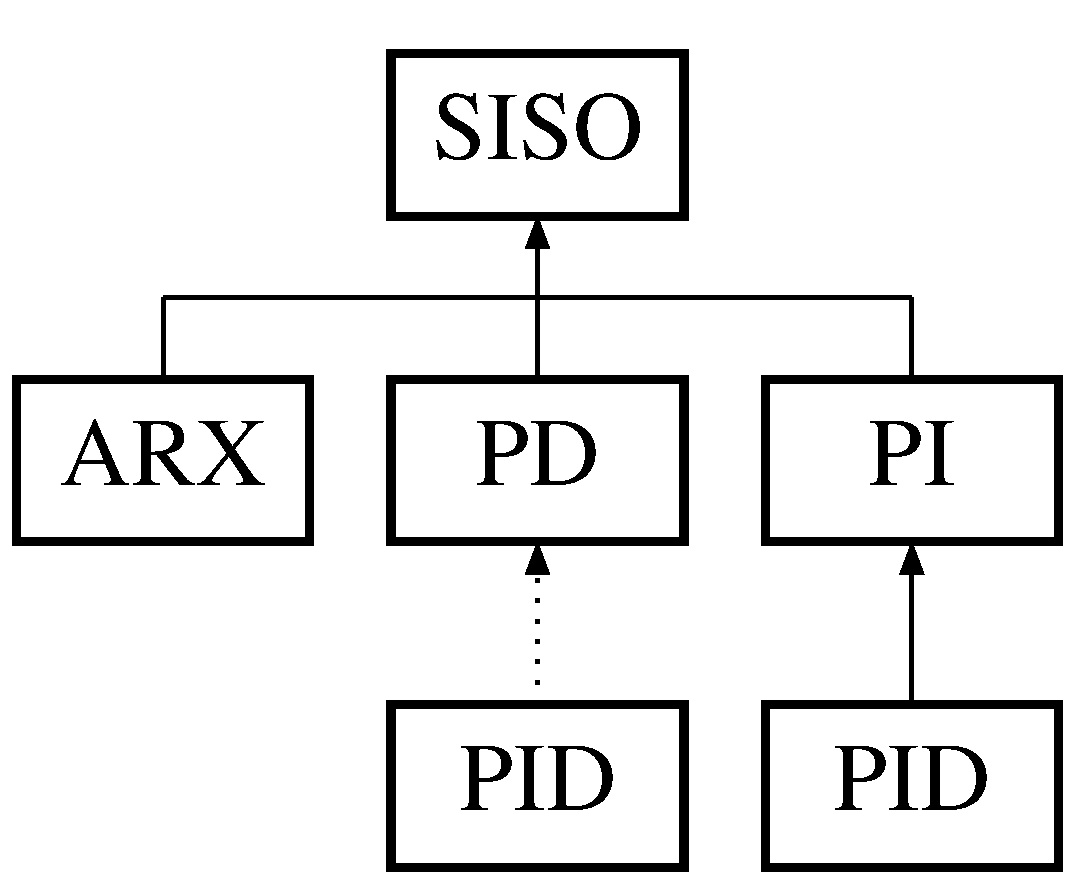
\includegraphics[height=4.000000cm]{class_s_i_s_o}
\end{center}
\end{figure}
\doxysubsection*{Metody publiczne}
\begin{DoxyCompactItemize}
\item 
virtual \mbox{\hyperlink{class_s_i_s_o_a3f6b0b7cda79493b941553e5d5780167}{$\sim$\+SISO}} ()
\begin{DoxyCompactList}\small\item\em Przez to, że klasa posiada jedynie metodę wirtualną, wirtualny musi być również destruktor. \end{DoxyCompactList}\end{DoxyCompactItemize}
\doxysubsubsection*{Metody publiczne dziedziczone z \mbox{\hyperlink{class_komponent___struktura}{Komponent\+\_\+\+Struktura}}}
\begin{DoxyCompactItemize}
\item 
virtual \mbox{\hyperlink{class_komponent___struktura_a3df8c1a1177bda3f17857ecef6ba2d6d}{$\sim$\+Komponent\+\_\+\+Struktura}} ()
\begin{DoxyCompactList}\small\item\em Wirtualny destruktor. \end{DoxyCompactList}\item 
void \mbox{\hyperlink{class_komponent___struktura_a0b11947c38aed479c984c20d32cc77c0}{Set\+Parent}} (\mbox{\hyperlink{class_komponent___struktura}{Komponent\+\_\+\+Struktura}} $\ast$nparent)
\begin{DoxyCompactList}\small\item\em Ustawienie danego \char`\"{}rodzica\char`\"{}. \end{DoxyCompactList}\item 
\mbox{\hyperlink{class_komponent___struktura}{Komponent\+\_\+\+Struktura}} $\ast$ \mbox{\hyperlink{class_komponent___struktura_a5eb3e69b28b2fb3ad8d761611a3e8927}{Get\+Parent}} () const
\begin{DoxyCompactList}\small\item\em Odebranie danego rodzica. \end{DoxyCompactList}\item 
virtual void \mbox{\hyperlink{class_komponent___struktura_afbe374b319f9be537bd65250173c0190}{dodaj}} (\mbox{\hyperlink{class_komponent___struktura}{Komponent\+\_\+\+Struktura}} $\ast$komponent)
\begin{DoxyCompactList}\small\item\em Operacja dodawania kolejnych \char`\"{}dzieci\char`\"{} do drzewa. W tym wypadku s� to obiekty \mbox{\hyperlink{class_s_i_s_o}{SISO}}. \end{DoxyCompactList}\item 
virtual void \mbox{\hyperlink{class_komponent___struktura_a9ebab0e681403b17baa7b9ba2579ecaa}{usun}} (\mbox{\hyperlink{class_komponent___struktura}{Komponent\+\_\+\+Struktura}} $\ast$komponent)
\begin{DoxyCompactList}\small\item\em Operacja usuni�cia kolejnych \char`\"{}dzieci\char`\"{} do drzewa. W tym wypadku s� to obiekty \mbox{\hyperlink{class_s_i_s_o}{SISO}}. \end{DoxyCompactList}\item 
virtual double \mbox{\hyperlink{class_komponent___struktura_a19686e69b56cee733d792af23e9237b7}{Symuluj}} (double s\+\_\+u)=0
\end{DoxyCompactItemize}
\doxysubsection*{Dodatkowe Dziedziczone Składowe}
\doxysubsubsection*{Atrybuty chronione dziedziczone z \mbox{\hyperlink{class_komponent___struktura}{Komponent\+\_\+\+Struktura}}}
\begin{DoxyCompactItemize}
\item 
\mbox{\hyperlink{class_komponent___struktura}{Komponent\+\_\+\+Struktura}} $\ast$ \mbox{\hyperlink{class_komponent___struktura_a7cb0e2ed12c6c2ecdfde465b1f1f4b54}{parent}}
\begin{DoxyCompactList}\small\item\em Wska�nik na klas� \mbox{\hyperlink{class_komponent___struktura}{Komponent\+\_\+\+Struktura}} wskazuj�ca na \char`\"{}rodzic�w\char`\"{}, czyli najstarsze elementy drzewa. \end{DoxyCompactList}\end{DoxyCompactItemize}


\doxysubsection{Opis szczegółowy}


Definicja w linii \mbox{\hyperlink{klasa_s_i_s_o_8hpp_source_l00009}{9}} pliku \mbox{\hyperlink{klasa_s_i_s_o_8hpp_source}{klasa\+SISO.\+hpp}}.



\doxysubsection{Dokumentacja konstruktora i destruktora}
\mbox{\Hypertarget{class_s_i_s_o_a3f6b0b7cda79493b941553e5d5780167}\label{class_s_i_s_o_a3f6b0b7cda79493b941553e5d5780167}} 
\index{SISO@{SISO}!````~SISO@{$\sim$SISO}}
\index{````~SISO@{$\sim$SISO}!SISO@{SISO}}
\doxysubsubsection{\texorpdfstring{$\sim$SISO()}{~SISO()}}
{\footnotesize\ttfamily virtual SISO\+::$\sim$\+SISO (\begin{DoxyParamCaption}{ }\end{DoxyParamCaption})\hspace{0.3cm}{\ttfamily [inline]}, {\ttfamily [virtual]}}



Przez to, że klasa posiada jedynie metodę wirtualną, wirtualny musi być również destruktor. 



Definicja w linii \mbox{\hyperlink{klasa_s_i_s_o_8hpp_source_l00012}{12}} pliku \mbox{\hyperlink{klasa_s_i_s_o_8hpp_source}{klasa\+SISO.\+hpp}}.



Dokumentacja dla tej klasy została wygenerowana z pliku\+:\begin{DoxyCompactItemize}
\item 
\mbox{\hyperlink{klasa_s_i_s_o_8hpp}{klasa\+SISO.\+hpp}}\end{DoxyCompactItemize}

\chapter{Dokumentacja plików}
\hypertarget{klasa_a_r_x_8cpp}{\section{Dokumentacja pliku klasa\-A\-R\-X.\-cpp}
\label{klasa_a_r_x_8cpp}\index{klasa\-A\-R\-X.\-cpp@{klasa\-A\-R\-X.\-cpp}}
}
{\ttfamily \#include \char`\"{}klasa\-S\-I\-S\-O.\-hpp\char`\"{}}\\*
{\ttfamily \#include \char`\"{}klasa\-A\-R\-X.\-hpp\char`\"{}}\\*
{\ttfamily \#include $<$iostream$>$}\\*
{\ttfamily \#include $<$fstream$>$}\\*
{\ttfamily \#include $<$vector$>$}\\*
{\ttfamily \#include $<$deque$>$}\\*
{\ttfamily \#include $<$numeric$>$}\\*
{\ttfamily \#include $<$random$>$}\\*
{\ttfamily \#include \char`\"{}json.\-hpp\char`\"{}}\\*
\subsection*{Definicje typów}
\begin{DoxyCompactItemize}
\item 
using \hyperlink{klasa_a_r_x_8cpp_ab701e3ac61a85b337ec5c1abaad6742d}{json} = nlohmann\-::json
\begin{DoxyCompactList}\small\item\em Wykorzystanie przestrzeni nazw \char`\"{}nlohmann\-::json\char`\"{}, używając wyłącznie \char`\"{}json\char`\"{}. \end{DoxyCompactList}\end{DoxyCompactItemize}
\subsection*{Funkcje}
\begin{DoxyCompactItemize}
\item 
void \hyperlink{klasa_a_r_x_8cpp_a73d9ecf1b45067ffeb02ce0f0e42ef43}{print} (std\-::vector$<$ double $>$ const \&input)
\begin{DoxyCompactList}\small\item\em Wyświetlenie kolejnych elementów wektora. \end{DoxyCompactList}\end{DoxyCompactItemize}


\subsection{Opis szczegółowy}
W pliku znajdują się zaimplementowane funkcje i konstruktory klasy \hyperlink{class_a_r_x}{A\-R\-X}, zadeklarowane w pliku nagłówkowym. Klasa \hyperlink{class_a_r_x}{A\-R\-X} dziedziczy funkcję Symuluj z klasy \hyperlink{class_s_i_s_o}{S\-I\-S\-O}, której implementacja znajduje się również w tym pliku. Poza tymi metodami w pliku można znaleźć dodatkowo funkcję print, umożliwiającą wyświetlenie elementów wektora. 

Definicja w pliku \hyperlink{klasa_a_r_x_8cpp_source}{klasa\-A\-R\-X.\-cpp}.



\subsection{Dokumentacja definicji typów}
\hypertarget{klasa_a_r_x_8cpp_ab701e3ac61a85b337ec5c1abaad6742d}{\index{klasa\-A\-R\-X.\-cpp@{klasa\-A\-R\-X.\-cpp}!json@{json}}
\index{json@{json}!klasaARX.cpp@{klasa\-A\-R\-X.\-cpp}}
\subsubsection[{json}]{\setlength{\rightskip}{0pt plus 5cm}using {\bf json} =  nlohmann\-::json}}\label{klasa_a_r_x_8cpp_ab701e3ac61a85b337ec5c1abaad6742d}


Wykorzystanie przestrzeni nazw \char`\"{}nlohmann\-::json\char`\"{}, używając wyłącznie \char`\"{}json\char`\"{}. 



Definicja w linii 20 pliku klasa\-A\-R\-X.\-cpp.



\subsection{Dokumentacja funkcji}
\hypertarget{klasa_a_r_x_8cpp_a73d9ecf1b45067ffeb02ce0f0e42ef43}{\index{klasa\-A\-R\-X.\-cpp@{klasa\-A\-R\-X.\-cpp}!print@{print}}
\index{print@{print}!klasaARX.cpp@{klasa\-A\-R\-X.\-cpp}}
\subsubsection[{print}]{\setlength{\rightskip}{0pt plus 5cm}void print (
\begin{DoxyParamCaption}
\item[{std\-::vector$<$ double $>$ const \&}]{input}
\end{DoxyParamCaption}
)}}\label{klasa_a_r_x_8cpp_a73d9ecf1b45067ffeb02ce0f0e42ef43}


Wyświetlenie kolejnych elementów wektora. 



Definicja w linii 168 pliku klasa\-A\-R\-X.\-cpp.


\hypertarget{klasa_a_r_x_8hpp}{}\doxysection{Dokumentacja pliku klasa\+ARX.\+hpp}
\label{klasa_a_r_x_8hpp}\index{klasaARX.hpp@{klasaARX.hpp}}
{\ttfamily \#include \char`\"{}klasa\+SISO.\+hpp\char`\"{}}\newline
{\ttfamily \#include $<$iostream$>$}\newline
{\ttfamily \#include $<$vector$>$}\newline
{\ttfamily \#include $<$deque$>$}\newline
\doxysubsection*{Komponenty}
\begin{DoxyCompactItemize}
\item 
class \mbox{\hyperlink{class_a_r_x}{ARX}}
\end{DoxyCompactItemize}


\doxysubsection{Opis szczegółowy}
Klasa \mbox{\hyperlink{class_a_r_x}{ARX}} dziedziczy metodę Symuluj z klasy interfejs \mbox{\hyperlink{class_s_i_s_o}{SISO}}. Jej zadaniem jest symulacja obiektu w postaci modelu \mbox{\hyperlink{class_a_r_x}{ARX}} 

Definicja w pliku \mbox{\hyperlink{klasa_a_r_x_8hpp_source}{klasa\+ARX.\+hpp}}.


\hypertarget{klasa_s_i_s_o_8hpp}{}\doxysection{Dokumentacja pliku klasa\+SISO.\+hpp}
\label{klasa_s_i_s_o_8hpp}\index{klasaSISO.hpp@{klasaSISO.hpp}}
\doxysubsection*{Komponenty}
\begin{DoxyCompactItemize}
\item 
class \mbox{\hyperlink{class_s_i_s_o}{SISO}}
\end{DoxyCompactItemize}


\doxysubsection{Opis szczegółowy}
Klasa \mbox{\hyperlink{class_s_i_s_o}{SISO}} stanowi klasę bazową w postaci interfejsu dla klas pochodnych. W jej skład wchodzi jedynie czysto wirtualna metoda Symuluj, zwracająca próbkę wyjścia, po podaniu na nią próbki wejścia. 

Definicja w pliku \mbox{\hyperlink{klasa_s_i_s_o_8hpp_source}{klasa\+SISO.\+hpp}}.


\hypertarget{_obiekt_dyskretny_lab_8cpp}{}\doxysection{Dokumentacja pliku Obiekt\+Dyskretny\+Lab.\+cpp}
\label{_obiekt_dyskretny_lab_8cpp}\index{ObiektDyskretnyLab.cpp@{ObiektDyskretnyLab.cpp}}
{\ttfamily \#include $<$iostream$>$}\newline
{\ttfamily \#include $<$vector$>$}\newline
{\ttfamily \#include $<$deque$>$}\newline
{\ttfamily \#include $<$fstream$>$}\newline
{\ttfamily \#include $<$locale$>$}\newline
{\ttfamily \#include \char`\"{}json.\+hpp\char`\"{}}\newline
{\ttfamily \#include \char`\"{}klasa\+ARX.\+hpp\char`\"{}}\newline
{\ttfamily \#include \char`\"{}klasa\+SISO.\+hpp\char`\"{}}\newline
{\ttfamily \#include \char`\"{}PI.\+hpp\char`\"{}}\newline
{\ttfamily \#include \char`\"{}PD.\+hpp\char`\"{}}\newline
{\ttfamily \#include \char`\"{}PID.\+hpp\char`\"{}}\newline
{\ttfamily \#include \char`\"{}funkcje\+Pomocniczne.\+hpp\char`\"{}}\newline
{\ttfamily \#include \char`\"{}Komponent.\+hpp\char`\"{}}\newline
{\ttfamily \#include \char`\"{}Komponent\+Konkretny.\+hpp\char`\"{}}\newline
{\ttfamily \#include \char`\"{}Dek\+Sin.\+hpp\char`\"{}}\newline
{\ttfamily \#include \char`\"{}Dek\+Szum.\+hpp\char`\"{}}\newline
{\ttfamily \#include \char`\"{}Dek\+Prost.\+hpp\char`\"{}}\newline
\doxysubsection*{Funkcje}
\begin{DoxyCompactItemize}
\item 
int \mbox{\hyperlink{_obiekt_dyskretny_lab_8cpp_ae66f6b31b5ad750f1fe042a706a4e3d4}{main}} ()
\end{DoxyCompactItemize}


\doxysubsection{Dokumentacja funkcji}
\mbox{\Hypertarget{_obiekt_dyskretny_lab_8cpp_ae66f6b31b5ad750f1fe042a706a4e3d4}\label{_obiekt_dyskretny_lab_8cpp_ae66f6b31b5ad750f1fe042a706a4e3d4}} 
\index{ObiektDyskretnyLab.cpp@{ObiektDyskretnyLab.cpp}!main@{main}}
\index{main@{main}!ObiektDyskretnyLab.cpp@{ObiektDyskretnyLab.cpp}}
\doxysubsubsection{\texorpdfstring{main()}{main()}}
{\footnotesize\ttfamily int main (\begin{DoxyParamCaption}{ }\end{DoxyParamCaption})}



Definicja w linii \mbox{\hyperlink{_obiekt_dyskretny_lab_8cpp_source_l00019}{19}} pliku \mbox{\hyperlink{_obiekt_dyskretny_lab_8cpp_source}{Obiekt\+Dyskretny\+Lab.\+cpp}}.


\hypertarget{_r_e_a_d_m_e_8md}{\section{Dokumentacja pliku R\-E\-A\-D\-M\-E.\-md}
\label{_r_e_a_d_m_e_8md}\index{R\-E\-A\-D\-M\-E.\-md@{R\-E\-A\-D\-M\-E.\-md}}
}

\addcontentsline{toc}{part}{Indeks}
\printindex
\end{document}
